\documentclass[journal,trans]{IEEEtran}

\usepackage[utf8]{inputenc}
\usepackage{graphicx}
\usepackage[spanish, es-tabla, activeacute]{babel}
\usepackage{verbatim}


\begin{document}

% Do not put math or special symbols in the title.
\newcommand{\titlepaper}{Diseño e Implementación de una ALU}

\title{\titlepaper}

\renewcommand\IEEEkeywordsname{Palabras clave}

\author{\IEEEauthorblockN{Emmanuel Naranjo-Blanco, Gabriel González-Rodríguez, Jose Fabio Navarro-Naranjo, Adrián Dittel-Retana, David Rodríguez-Camacho}

\IEEEauthorblockA{naranjo760emm@estudiantec.cr}
\IEEEauthorblockA{gabrielgr01@estudiantec.cr}
\IEEEauthorblockA{emailEstudiante2@estudiantec.cr}
\IEEEauthorblockA{emailEstudiante2@estudiantec.cr}
\IEEEauthorblockA{emailEstudiante2@estudiantec.cr}
\IEEEauthorblockA{\\Área Académica de Ingeniería Mecatrónica}
\IEEEauthorblockA{\\Instituto Tecnológico de Costa Rica}
}

% The paper headers
\markboth{Naranjo, González, Navarro, Dittel, Rodríguez, \titlepaper}%
{Shell \MakeLowercase{\textit{et al.}}: Bare Demo of IEEEtran.cls for Journals}

\IEEEtitleabstractindextext{%
\begin{abstract}

La Unidad Aritmética Lógica (ALU) consiste en una parte esencial de la unidad central de procesamiento, encargada de realizar operaciones lógicas y aritméticas para cumplir instrucciones dentro de un sistema computacional. En el presente proyecto de laboratorio se presentará una propuesta para el diseño de una ALU que lleva a cabo siete operaciones (lógicas y matemáticas), además de los resultados obtenidos tras su ejecución. La solución a la propuesta se basó fundamentalmente en el uso de lógica combinacional, y a nivel de diseño se utilizó el método de diseño modular, en donde se divide le sistema en subsistemas más pequeños, llamados módulos, a los cuales se les encuentra una solución individual, y reutilizable.  Posteriormente se integran las soluciones para cada módulo y se le agregan las distintas banderas como parte de las restricciones del proyecto. Una vez finalizado el experimento, se llega a la conclusión principal del proyecto: Se verificó mediante el lenguaje de descripción de hardware (HDL), y su implementación en la placa de desarrollo BASYS 3, el correcto funcionamiento de la ALU propuesta mediante la estructura de diseño planteada. Además, de la simulación se obtuvo un bajo consumo de potencia (5.576W) y un LUT del 1\%, lo que significa que hubo un bajo consumo de área.


\end{abstract}

\begin{IEEEkeywords}
Diseño modular, FPGA, Lógica Combinacional, Verilog.
\end{IEEEkeywords}}

\maketitle
\IEEEdisplaynontitleabstractindextext
\IEEEpeerreviewmaketitle

\section{INTRODUCCIÓN}

Parte fundamental de la electrónica digital consiste en la implementación de los conocimientos en la integración de sistemas completamente funcionales y aplicables para solucionar problemas de la vida real. En el presente proyecto de laboratorio se pretende aplicar la teoría, específicamente aquella relacionada con lógica combinacional, para así emplearla de forma práctica en una Unidad Aritmética Lógica (ALU, por sus siglas en inglés). 

De acuerdo con Tocci, una ALU consiste en un circuito que permite realizar operaciones lógicas y aritméticas \cite{Tocci}. Las cuales se encuentran como parte fundamental de los sistemas tecnológicos actuales como computadoras, celulares y tablets. A su vez, existen presentaciones en circuitos integrados como los chips 74LS382 o 74HC382 cuyo bloque se representa en la Figura \ref{fig:ALU}. 

En este tipo de chips se basa el objetivo específico del proyecto, el cual consiste en implementar un sistema lógico en un ambiente de verificación de hardware. Donde como parte de los objetivos generales se tiene comprender el proceso de diseño y verificación de los sistemas digitales, y aplicar el diseño en una placa de desarrollo. Para este caso se utiliza una matriz de puertas lógicas programable en campo, comúnmente llamada FPGA (field-programmable gate array).

\begin{figure}[!h]
	\centering
	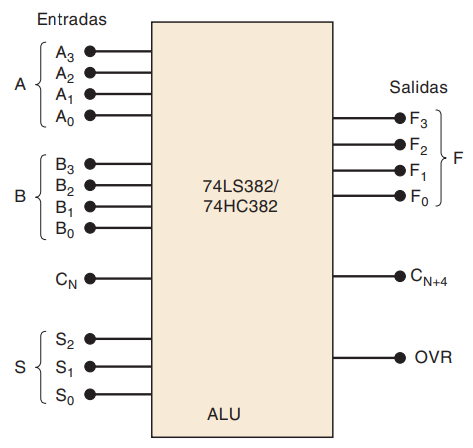
\includegraphics[width =0.7 \columnwidth]{Imagenes/ALU}
	\caption{Símbolo de bloque para el chip ALU 74LS382/HC382 \cite{Tocci}.}
	\label{fig:ALU}
\end{figure}

La idea fundamental de este proyecto consiste en diseñar una ALU que realice todas las operaciones descritas en la Tabla \ref{tab:operaciones}. Para esto se tienen dos entradas de datos A y B, y una salida Y, todas con un tamaño constante de palabra de 6 bits y operando bajo el sistema de complemento a dos. Además, las operaciones se escogen mediante un selector SEL de 3 bits y se requiere de tres banderas: cero, paridad par y desbordamiento. 

\begin{table}[!h]
  \begin{center}
    \caption{Descripción de las operaciones de la ALU por diseñar.}
    \label{tab:operaciones}
    \begin{tabular}{c | c | c }
      \hline
      SEL [2:0] & Tipo de Operación & Y \\
      \hline
       000 & XOR & Y = A $\string^$ B \\
       \hline
       001 & AND & Y = A $\&$ B \\
       \hline
       010 & OR & Y = A $\mid$ B \\
       \hline
       011 & Desplazamiento lógico a la derecha & Y=A $\gg$ 1 \\
       \hline
       100 & Suma con signo & Y = A + B \\
       \hline
       101 & Multiplicación con signo & Y = A * B \\
       \hline
       110 & Resta con signo & Y = A - B \\
       \hline
       111 & Quintuplicado de un número & Y = 5 * A \\
      \hline
    \end{tabular}
  \end{center}
\end{table}

Para simular e implementar el diseño propuesto se utiliza la placa BASYS 3 Artix-7 (xc7a35tcpg236-2L), la cual se programa en Verilog, un lenguaje de descripción de hardware (HDL, por sus siglas en inglés) al cual se le realiza una previa simulación para comprobar su correcto funcionamiento.

A modo conceptual, un HDL se trata de un lenguaje de programación para modelar un bloque de hardware, el cual permite simular la operación del circuito antes de fabricarlo \cite{Paulino}. En este caso, se trabajó con el HDL Verilog debido a su popularidad y simplicidad, y por ser estándar en la industria de las FPGA. Para esto, cada componente se describe con módulos y la verificación de este se establece bajo la estructura de un TestBench.

En las siguientes secciones se detallará el proceso de diseño junto con los diagramas modulares realizados y su descripción. Posteriormente se analizarán los resultados obtenidos tanto a nivel físico como simulado mediante el software Vivado. 


\section{DISEÑO DE LA ALU}

A continuación se describe el proceso realizado para el diseño de la ALU anteriormente descrita.

%% Primer nivel


%% 

%% Esto se tomó del  abstract, siento que es muy específico para utilizarlo ahí, pero puede usarse ya en la sección donde se describe el diseño
\begin{comment}
Parte del problema por resolver consiste en el uso de componentes combinacionales, para lo cual se dispuso de un multiplexor de ocho entradas como el encargado de gobernar las operaciones.

se realizó una partición por módulos, lo cual consiste en estructurar la descripción del proyecto en secciones definidas, cada una con su respectivo proceso de diseño y codificación en el HDL Verilog.

Posteriormente se integró cada solución propuesta en un proyecto principal denominado main, al cual se le ajustaron los cambios correspondientes y se le agregó las distintas banderas como parte de las restricciones del proyecto.
\end{comment}
%%

\section{IMPLEMENTACIÓN Y ANÁLISIS DE RESULTADOS}


\section{CONCLUSIONES}
A partir de este presente trabajo, se logró concluir lo siguiente.
\begin{itemize}
    \item El diseño modular consiste en un mecanismo ventajoso debido a que facilita la construcción de sistemas digitales de mayor complejidad. Además, facilita la depuración en caso de cometer un error.
\end{itemize}

\section{RECOMENDACIONES}
Para realizar exitosamente el proyecto es necesario cumplir una serie de recomendaciones.
\begin{itemize}
    \item Es indispensable la partición del problema en subsistemas por dos razones, para familiarizarse con los estándares de diseño y comprender el proceso de solucionar sistemas digitales complejos que por medio de otras herramientas como tablas de verdad o funciones lógicas no se podría, o se volvería innecesariamente complicado.
\end{itemize}




%%%%%%%%%%%%%%%%%%%%%%%%%%%%%%%%%%%%%%%%%
\begin{comment}

Ejemplos:

\begin{table}[htb]
  \begin{center}
    \caption{Filter bank's output's STD error per band for an impulsive input signal, tested against BeagleBoard's output for the same input signal. Worst case is band 5, close to a 4\% STD error.}
    \label{tab:filter-error}
    \begin{tabular}{c | c | c | c | c | c }
      \hline
      Band & 1 & 2 & 3 & 4 & 5 \\
      \hline
       STD & 0.0090 & 0.0097 & 0.0166 & 0.0291 & 0.0389 \\
      \hline
    \end{tabular}
  \end{center}
\end{table}


\begin{figure}[hbtp]
	\centering
	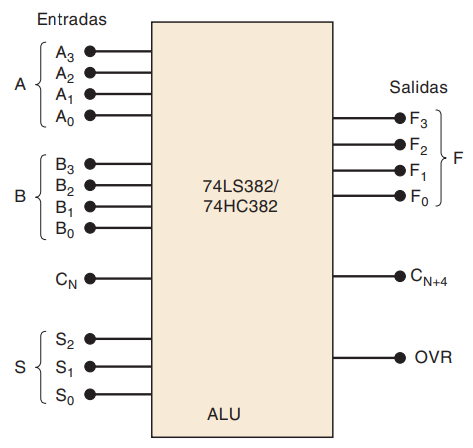
\includegraphics[width = \columnwidth]{Imagenes/ALU}
	\caption[]{Sample of results from bands 1 and 8 from the Verilog version of the filter bank, compared against data from the BeagleBoard's filter version.}
	\label{fig:FiguraCircuito}
\end{figure}

\end{comment}

%%%%%%%%%%%%%%%%%%%%%%%%%%%%%%%%%%%%%%%%%%%

\begin{thebibliography}{1}

\bibitem{Tocci}
R. Tocci. \emph{Sistemas digitales: Principios y aplicaciones}. Décima edición. Pearson Education. 2007.

\bibitem{Paulino}
Paulino Ruiz de Clavijo Vásquez. \emph{Introducción a HDL Verilog - Presentaciones de clase}. Departamento de Tecnología Electrónica. Universidad de Sevilla.



\end{thebibliography}

\end{document}
